\subsubsection{Use Cases}
In the following section we will present the use case diagram and the use cases made to uncover the functional requirements for the system.

\subsubsubsection{Use case diagram}
We have produced a use case diagram, see Figure \ref{useCaseImg} p. \pageref{useCaseImg}, which outlines the boundaries of the system, and how the different actors (user types) can interact with the server. 
\begin{figure}[h]
\centering
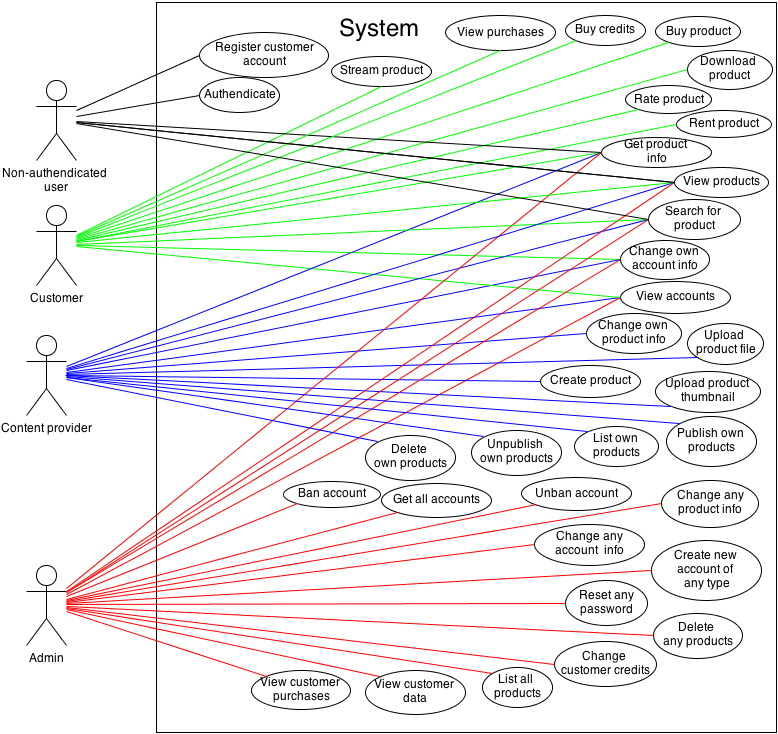
\includegraphics[scale=0.5]{illustrations/UseCaseDiagram.png}
\caption{Use case diagram for our web service}
\label{useCaseImg}
\end{figure}

\subsubsubsection{Use cases}
In the following section use cases for our system will be listed. Every use case will have a short description of the scenario the use case is representing, if there are any pre- or postconditions these will be mentioned and then the basic flow and success scenario will be listed.\\
\textit{Only two use cases will be listed here. For a complete list of our use cases, see\apref{Apendix_usecases}}

\textbf{Success scenario: Register new user} \\
Jane Doe wants to register and become a customer. 
\begin{tabbing}
\hspace{5mm}\=\hspace{28mm}\=\kill
\>Primary Actor:\> Non-registered user\\
\>Precondition:\> -\\
\>Postcondition:\> A new customer account is created, and the user is logged in.
\end{tabbing}
\begin{enumerate} \setlength{\itemsep}{-1mm}
	\item Jane Doe clicks the "register" link.
	\item Jane Doe enters the required information (email, username and password).
	\item Jane Doe submits the request
\end{enumerate}
% % %
\vspace{3mm}
\textbf{Success scenario: Show product} \\
Jane Doe wants see what products there are available with the genre "Action".
\begin{tabbing}
\hspace{5mm}\=\hspace{26mm}\=\kill
\>Primary Actor:\> All actors\\
\>Precondition:\> -\\
\>Postcondition:\> -
\end{tabbing}
\begin{enumerate} \setlength{\itemsep}{-1mm}
	\item Jane Doe searches for the category "Action".
	\item She browse the returned list, and clicks on one of the titles to see more.
	\item Jane Doe is presented with a more detailed view of the chosen product.
\end{enumerate}
% % %
\vspace{3mm}
\textbf{Success scenario: Log in} \\
John doe wants to log in to his account. 
\begin{tabbing}
\hspace{5mm}\=\hspace{26mm}\=\kill
\>Primary Actor:\> Customer, Content Provider and Admin\\
\>Precondition:\> The actor already has an account\\
\>Postcondition:\> The actor is logged in with her account.
\end{tabbing}
\begin{enumerate} \setlength{\itemsep}{-1mm}
	\item John Doe click on the "log in" link.
	\item John Doe enters his login information (username/email and password).
	\item John doe clicks the "enter" link.
\end{enumerate}
% % %
\vspace{3mm}
\textbf{Success scenario: Manage account} \\
John doe wants to edit his account information.
\begin{tabbing}
\hspace{5mm}\=\hspace{26mm}\=\kill
\>Primary Actor:\> Customer and Content Provider\\
\>Precondition:\> The actor is logged in\\
\>Postcondition:\> The actor has changed his/hers account information.
\end{tabbing}
\begin{enumerate} \setlength{\itemsep}{-1mm}
	\item John Doe goes to his account-page.
	\item John Doe changes the data his wishes to be changed.
	\item John doe clicks the "save" link.
\end{enumerate}
% % %
\vspace{3mm}
\textbf{Success scenario: Log in} \\
John doe wants to log in to his account. 
\begin{tabbing}
\hspace{5mm}\=\hspace{26mm}\=\kill
\>Primary Actor:\> Customer, Content Provider and Admin\\
\>Precondition:\> The actor already has an account\\
\>Postcondition:\> The actor is logged in.
\end{tabbing}
\begin{enumerate} \setlength{\itemsep}{-1mm}
	\item John Doe click on the "log in" link.
	\item John Doe enters his login information (username/email and password).
	\item John doe clicks the "enter" link.
\end{enumerate}
% % %
\vspace{3mm}
\textbf{Success scenario: Log out} \\
John doe wants to log out of his account. 
\begin{tabbing}
\hspace{5mm}\=\hspace{26mm}\=\kill
\>Primary Actor:\> Customer, Content Provider and Admin\\
\>Precondition:\> The actor is already logged in\\
\>Postcondition:\> The actor is logged off his/hers account.
\end{tabbing}
\begin{enumerate} \setlength{\itemsep}{-1mm}
	\item John Doe click on the "log out" link.
\end{enumerate}
% % %
\vspace{3mm}
\textbf{Success scenario: Rent product} \\
Spiderman wants to rent the movie "The Dark Knight Rises". 
\begin{tabbing}
\hspace{5mm}\=\hspace{26mm}\=\kill
\>Primary Actor:\> Customer\\
\>Precondition:\> The actor is logged in and it is possible to rent the product.\\
\>Postcondition:\> The actor has rented the product and the credits is withdrawn from the actor's account.
\end{tabbing}
\begin{enumerate} \setlength{\itemsep}{-1mm}
	\item Spiderman navigates to the movie.
	\item He clicks the "rent product" link.
	\item He confirms that he will spend 50 credits to rent this product for a week.
\end{enumerate}
% % %
\vspace{3mm}
\textbf{Success scenario: Buy product} \\
Spiderman wants to buy the movie "The Dark Knight". 
\begin{tabbing}
\hspace{5mm}\=\hspace{26mm}\=\kill
\>Primary Actor:\> Customer\\
\>Precondition:\> The actor is logged in and it is possible to buy the product.\\
\>Postcondition:\> The actor has bought the product and the credits is withdrawn from the actors account.
\end{tabbing}
\begin{enumerate} \setlength{\itemsep}{-1mm}
	\item Spiderman navigates to the movie.
	\item He clicks the "buy product" link.
	\item He confirms that he will spend 100 credits to buy this product.
\end{enumerate}
% % %
\vspace{3mm}
\textbf{Success scenario: Rate product} \\
Spiderman wants to rate the movie "The Dark Knight". 
\begin{tabbing}
\hspace{5mm}\=\hspace{26mm}\=\kill
\>Primary Actor:\> Customer\\
\>Precondition:\> The actor is logged in and it's possible to buy the product.\\
\>Postcondition:\> The actor has bought the product and the credits is withdrawn from the actors account.
\end{tabbing}
\begin{enumerate} \setlength{\itemsep}{-1mm}
	\item Spiderman navigates to the movie.
	\item He rates the product on a scale from -5 to 5.
\end{enumerate}
% % %
\vspace{3mm}
\textbf{Success scenario: Create new product} \\
Claus wants to create a new product. 
\begin{tabbing}
\hspace{5mm}\=\hspace{26mm}\=\kill
\>Primary Actor:\> Content Provider\\
\>Precondition:\> The actor is logged in.\\
\>Postcondition:\> The actor has created a new un-published product without an associated media file.
\end{tabbing}
\begin{enumerate} \setlength{\itemsep}{-1mm}
	\item Claus clicks the "Create product" link.
	\item He inserts the requested data.
	\item He clicks the "create" link.
\end{enumerate}
% % %
\vspace{3mm}
\textbf{Success scenario: Add media to a product} \\
Claus wants to add a movie to his newly created product.
\begin{tabbing}
\hspace{5mm}\=\hspace{26mm}\=\kill
\>Primary Actor:\> Content Provider\\
\>Precondition:\> The actor is logged in and has a product without any media.\\
\>Postcondition:\> The actor has uploaded the media and the product is published.
\end{tabbing}
\begin{enumerate} \setlength{\itemsep}{-1mm}
	\item Claus navigates to the product.
	\item He clicks the "add media" link.
	\item He chooses the media from his local computer and clicks the "upload" link.
\end{enumerate}
% % %
\vspace{3mm}
\textbf{Success scenario: Edit product information} \\
Claus wants to edit information about one of his products.
\begin{tabbing}
\hspace{5mm}\=\hspace{26mm}\=\kill
\>Primary Actor:\> Content Provider and Admin\\
\>Precondition:\> The actor is logged in. If actor is a Content Provider, she needs to own the product\\
\>Postcondition:\> The actor has change the information about the product.
\end{tabbing}
\begin{enumerate} \setlength{\itemsep}{-1mm}
	\item Claus navigates to the product he wants to change.
	\item He changes the information.
	\item He clicks the "save" link.
\end{enumerate}
% % %
\vspace{3mm}
\textbf{Success scenario: Unpublish a product} \\
Claus wants to unpublish one of his products.
\begin{tabbing}
\hspace{5mm}\=\hspace{26mm}\=\kill
\>Primary Actor:\> Content Provider and Admin\\
\>Precondition:\> The actor is logged in and the product has be to published. If actor is a Content Provider, she needs to own the product\\
\>Postcondition:\> The product is unpublished.
\end{tabbing}
\begin{enumerate} \setlength{\itemsep}{-1mm}
	\item Claus navigates to the product he wants to unpublish.
	\item He clicks the "unpublish" link.
\end{enumerate}
% % %
\vspace{3mm}
\textbf{Success scenario: Publish a product} \\
Claus wants to publish one of his products.
\begin{tabbing}
\hspace{5mm}\=\hspace{26mm}\=\kill
\>Primary Actor:\> Content Provider and Admin\\
\>Precondition:\> The actor is logged in and the product has be to unpublished and be associated with a media. If actor is a Content Provider, she needs to own the product\\
\>Postcondition:\> The product is published.
\end{tabbing}
\begin{enumerate} \setlength{\itemsep}{-1mm}
	\item Claus navigates to the product he wants to publish.
	\item He clicks the "publish" link.
\end{enumerate}
% % %
\vspace{3mm}
\textbf{Success scenario: Change information about a specific Customer, Content Provider or Admin} \\
Morten wants to change Spidermans account information.
\begin{tabbing}
\hspace{5mm}\=\hspace{26mm}\=\kill
\>Primary Actor:\> Admin\\
\>Precondition:\> The actor is logged in.\\
\>Postcondition:\> The actor has changed the information about the wished account.
\end{tabbing}
\begin{enumerate} \setlength{\itemsep}{-1mm}
	\item Morten navigates to Spiderman's profile-page.
	\item He make the wished changes.
	\item He clicks the "save" link.
\end{enumerate}
% % %
\vspace{3mm}
\textbf{Success scenario: Ban a specific account} \\
Morten wants to ban Claus' account.
\begin{tabbing}
\hspace{5mm}\=\hspace{26mm}\=\kill
\>Primary Actor:\> Admin\\
\>Precondition:\> The actor is logged in, the other action is not already banned, neither is the account in question the admin himself.\\
\>Postcondition:\> The actor has banned the account in question.
\end{tabbing}
\begin{enumerate} \setlength{\itemsep}{-1mm}
	\item Morten navigates to Claus' profile-page.
	\item Morten clicks the "ban" link.
	\item He confirms his action.
\end{enumerate}
% % %
\vspace{3mm}
\textbf{Success scenario: Unban a specific account} \\
Morten wants to unban Claus' account.
\begin{tabbing}
\hspace{5mm}\=\hspace{26mm}\=\kill
\>Primary Actor:\> Admin\\
\>Precondition:\> The actor is logged in, the other action is banned, and the account in question is not the admin himself.\\
\>Postcondition:\> The actor has unbanned the account in question.
\end{tabbing}
\begin{enumerate} \setlength{\itemsep}{-1mm}
	\item Morten navigates to Claus' profile-page.
	\item Morten clicks the "unban" link.
	\item He confirms his action.
\end{enumerate}
% % %
\vspace{3mm}
\textbf{Success scenario: Create new account} \\
Morten wants to create a new account.
\begin{tabbing}
\hspace{5mm}\=\hspace{26mm}\=\kill
\>Primary Actor:\> Admin\\
\>Precondition:\> The actor is logged in.\\
\>Postcondition:\> A new account is created.
\end{tabbing}
\begin{enumerate} \setlength{\itemsep}{-1mm}
	\item Morten opens the "create new account" page
	\item Morten fills in the form.
	\item He clicks the "save" link.
\end{enumerate}